\documentclass{beamer}
\usepackage{fontspec,xunicode,xltxtra,beamerthemesplit}
\usepackage{graphicx}
\usepackage{beamerthemeshadow}
%\usepackage{algorithmic}
%\usepackage{algorithm}
\usepackage[CJKmath = true]{xeCJK}
\usepackage{fancyhdr}

\usetheme{Antibes}
%\setsansfont[Mapping=tex-text]{SimSun}
%\setmainfont[BoldFont=Microsoft YaHei]{SimSun}
%\setmonofont{Microsoft YaHei}
\setCJKmainfont[BoldFont=Microsoft YaHei]{SimSun}
%\setCJKmainfont{SimSun}
%\setCJKmathfont{楷体}
%\setCJKsansfont{Times New Roman}


\title{RBM and DBN}
\author{赵惜墨}
\date{\today}
\institute{哈尔滨工业大学\\计算机学院\\智能技术与自然语言处理实验室}

\XeTeXlinebreaklocale "zh" % 表示用中文的断行
\XeTeXlinebreakskip = 0pt plus 1pt % 多一点调整的空间

\begin{document}

\section{介绍}

\frame{\titlepage}

\frame{
\frametitle{优点}
\begin{enumerate}
\item 保留了bp利用梯度方法调整权重的有效性、简单性
\item 学习$P(image)$而不是$P(label|image)$
\end{enumerate}

}

\frame{
  \frametitle{belief nets}
  \begin{columns}
    \begin{column}{0.5\textwidth}
      \begin{figure}
        \centering
        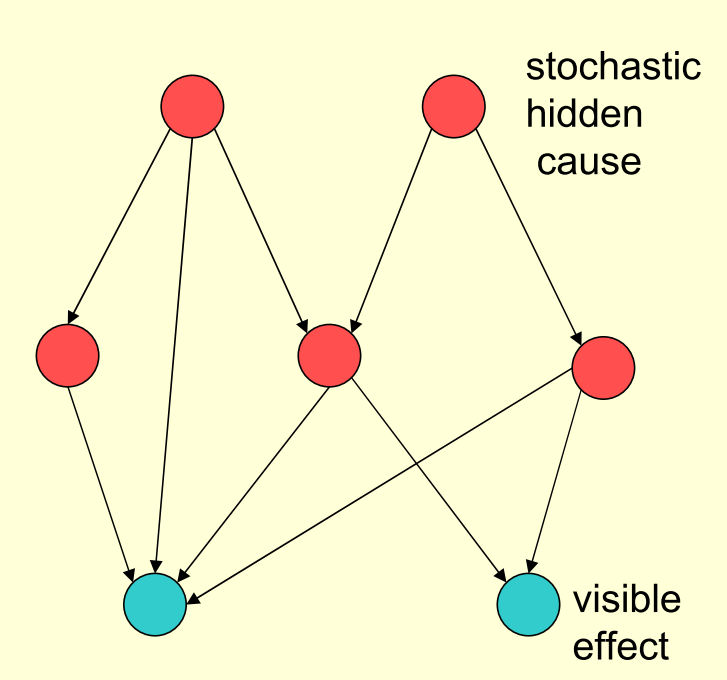
\includegraphics[height=5cm,width=6cm]{beliefnets.png}
        \label{fig:viterbi}
      \end{figure}
    \end{column}
    \begin{column}{0.5\textwidth}
      \begin{enumerate}
      \item 置信网由一个具有随机变量的有向图构成
      \item 通过观测可见节点,解决以下两个问题
        \begin{enumerate}
        \item 推理问题:解决未观察到的节点的状态
        \item 学习问题:通过调整可见节点相互之间的关系使网络产生更正确的观测变量
        \end{enumerate}
        
      \end{enumerate}
    \end{column}
  \end{columns}
  
}

\frame{
\frametitle{表示、学习}
logistic belief net 由二元随机变量组成。
\begin{displaymath}
  p(s_i =1 ) = \frac{1}{1+\exp(-b_i - \sum_j s_j w_{ji})}
\end{displaymath}

% 作者的想法是,后验分布是有相关性的,其先验是独立的,相关部分由似然产生。可以添加一个“补充”的先验,来消除似然部分的相关性。

\begin{displaymath}
  \Delta W_{ji} = \epsilon s_j (s_i - p_i)
\end{displaymath}

\begin{figure}
  \centering
  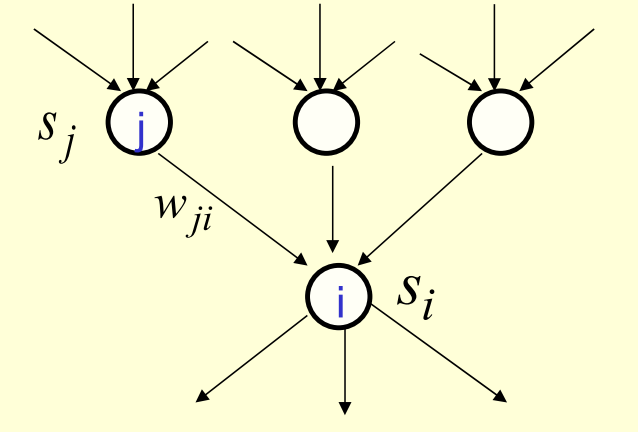
\includegraphics[height=4cm,width=6cm]{learningbelief.png}

  \label{fig:viterbi}
\end{figure}

}

\frame{
  \frametitle{explaining away}

  即使两个隐含变量独立,在两个变量都能影响到的事件上,它们也能变得相关。

  发生地震减弱了发生卡车把房子撞了
\begin{figure}
  \centering
  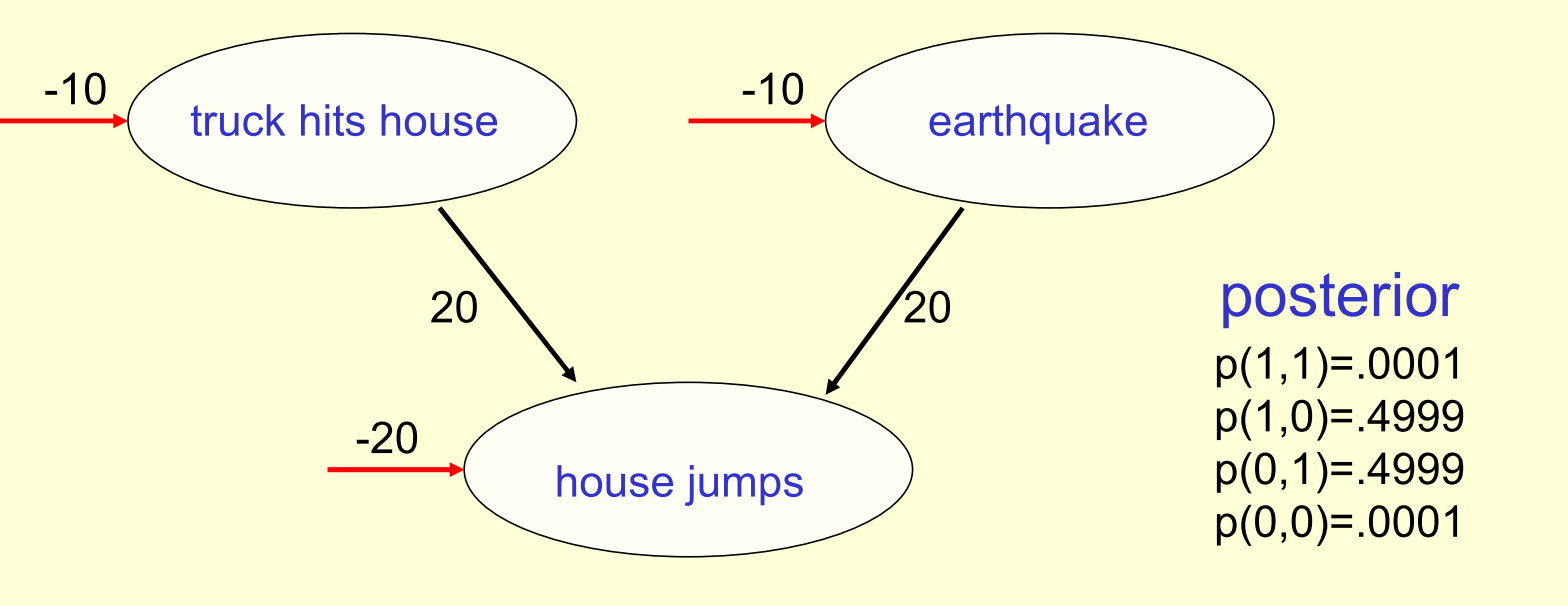
\includegraphics[height=4cm,width=9cm]{explainaway.png}

  \label{fig:viterbi}
\end{figure}

explaining away 使有向图推理更困难了。

}

\frame{
  \frametitle{一次学习一层参数所带来的问题}

  \begin{columns}
    \begin{column}{0.4\textwidth}
      \begin{figure}
        \centering
        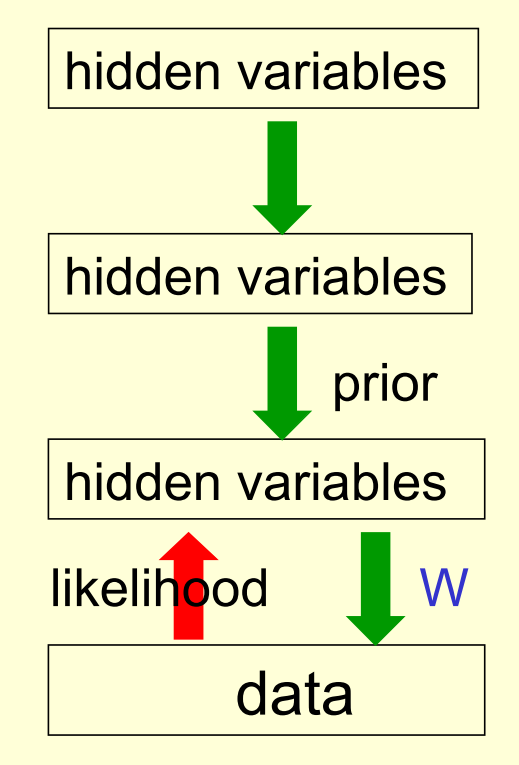
\includegraphics[height=5cm,width=4cm]{problem.png}
        \label{fig:viterbi}
      \end{figure}
    \end{column}
    \begin{column}{0.6\textwidth}
        \begin{itemize}
        \item 为了学习W(权重),需要学习第一层隐含层的后验分布
        \end{itemize}
          \begin{description}
          \item[问题1] 由于“explaining away”,学习会变得非常复杂
          \item[问题2] 后验既依赖于先验也依赖于似然,所以为了学习(W),需要知道更高层的参数,所有的权重都相关。
          \end{description}
    \end{column}
  \end{columns}

}



\section{complementary priors}



\frame{
\frametitle{可以采用的学习方法}
\begin{itemize}
\item MCMC:费时
\item 变分:不准确
\end{itemize}
}


\frame{
\frametitle{DBN所带来的突破}
\begin{enumerate}
\item 为了高效的学习,需要一次学一层。但是在假设隐含变量独立的情况写学习效果不好。
  \begin{itemize}
  \item 隐含变量后验分布不独立导致对于非线性模型的推理十分的困难。
  \item 在学习的过程中,算法在隐含层中寻找独立的解释,但是实际情况并非如此。
  \end{itemize}

\item 为了解决这些问题,引入了无向图模型。
\end{enumerate}
}

\frame{
  \frametitle{RBM}

   \begin{columns}
    \begin{column}{0.4\textwidth}
      \begin{figure}
        \centering
        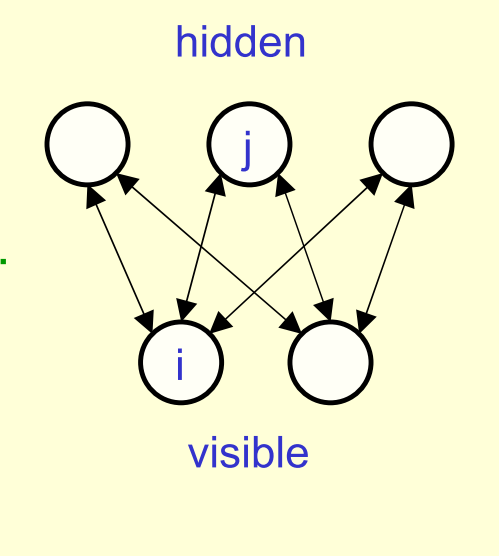
\includegraphics[height=5cm,width=5cm]{rbm.png}
        \label{fig:viterbi}
      \end{figure}
    \end{column}
    \begin{column}{0.6\textwidth}
      \begin{itemize}
      \item 对于连接进行限制,只有一层
      \item 隐含层之间没有联系
      \item 给定可见节点,隐含层间节点相互独立
      \end{itemize}
    \end{column}
  \end{columns}
  
}

\frame{
\frametitle{能量}
\begin{displaymath}
  E(v,h) = - \sum_{i,j} v_i h_j w_{ij}
\end{displaymath}
\begin{displaymath}
  - \frac{\partial E(v,h)}{\partial w_{ij}} = v_i h_j
\end{displaymath}

}

\frame{
  \frametitle{能量->概率}

  \begin{enumerate}
  \item 每一个可能的可见节点和隐含节点的组合都有一个能量
  \item 能量决定概率
    \begin{displaymath}
      p(v,h) = \frac{ e^{-E(v,h)}}{\sum_{u,g} e^{-E(u,g)}}
    \end{displaymath}

  \item 可见节点的概率是所有含有该可见节点的组合的加和
    \begin{displaymath}
      p(v) = \frac{\sum_h e^{-E(v,h)}}{\sum_{u,g} e^{-E(u,g)}}
    \end{displaymath}
    
  \end{enumerate}
}

\frame{
\frametitle{MLE learning for RBM}
      \begin{figure}
        \centering
        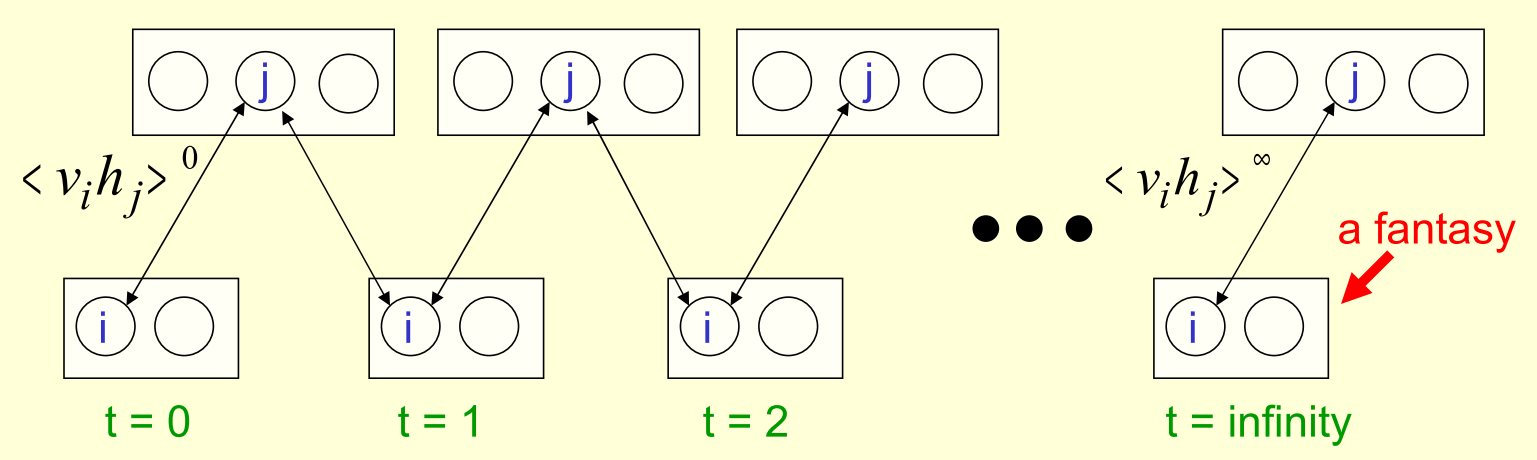
\includegraphics[height=4cm,width=10cm]{MLERBM.png}
        \label{fig:viterbi}
      \end{figure}

      \begin{displaymath}
        \frac{\partial \log p(v)}{\partial w_{ij}} = <v_i h_j>^0 - <v_i h_j>^{\infty}
      \end{displaymath}
}

\frame{
  \frametitle{quick way}

   \begin{columns}
    \begin{column}{0.5\textwidth}
      \begin{figure}
        \centering
        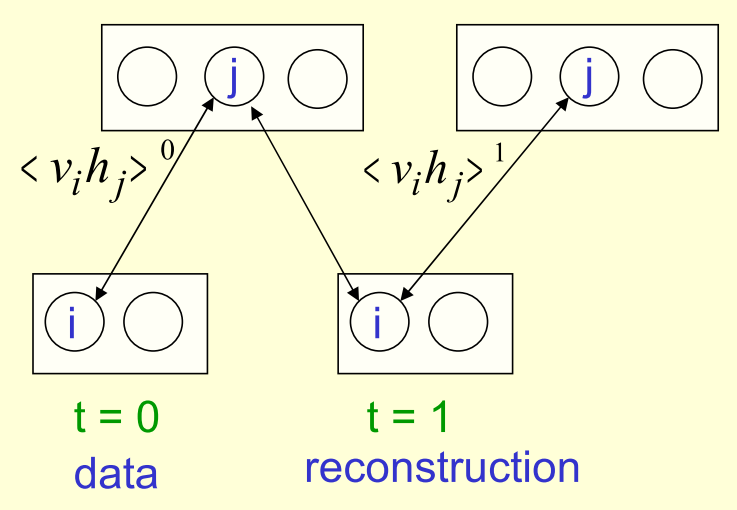
\includegraphics[height=5cm,width=6cm]{quickway.png}
        \label{fig:viterbi}
      \end{figure}
    \end{column}
    \begin{column}{0.5\textwidth}
      \begin{itemize}
      \item 从观测节点开始
      \item 更新隐含节点
      \item 重建可见节点
      \item 再次更新隐含节点
      \end{itemize}
      \begin{displaymath}
        \Delta w_{ij} = \epsilon (<v_i h_j>^0 - <v_i h_j>^{1})
      \end{displaymath}
    \end{column}
  \end{columns}

}

\frame{
\frametitle{例子}
      \begin{figure}
        \centering
        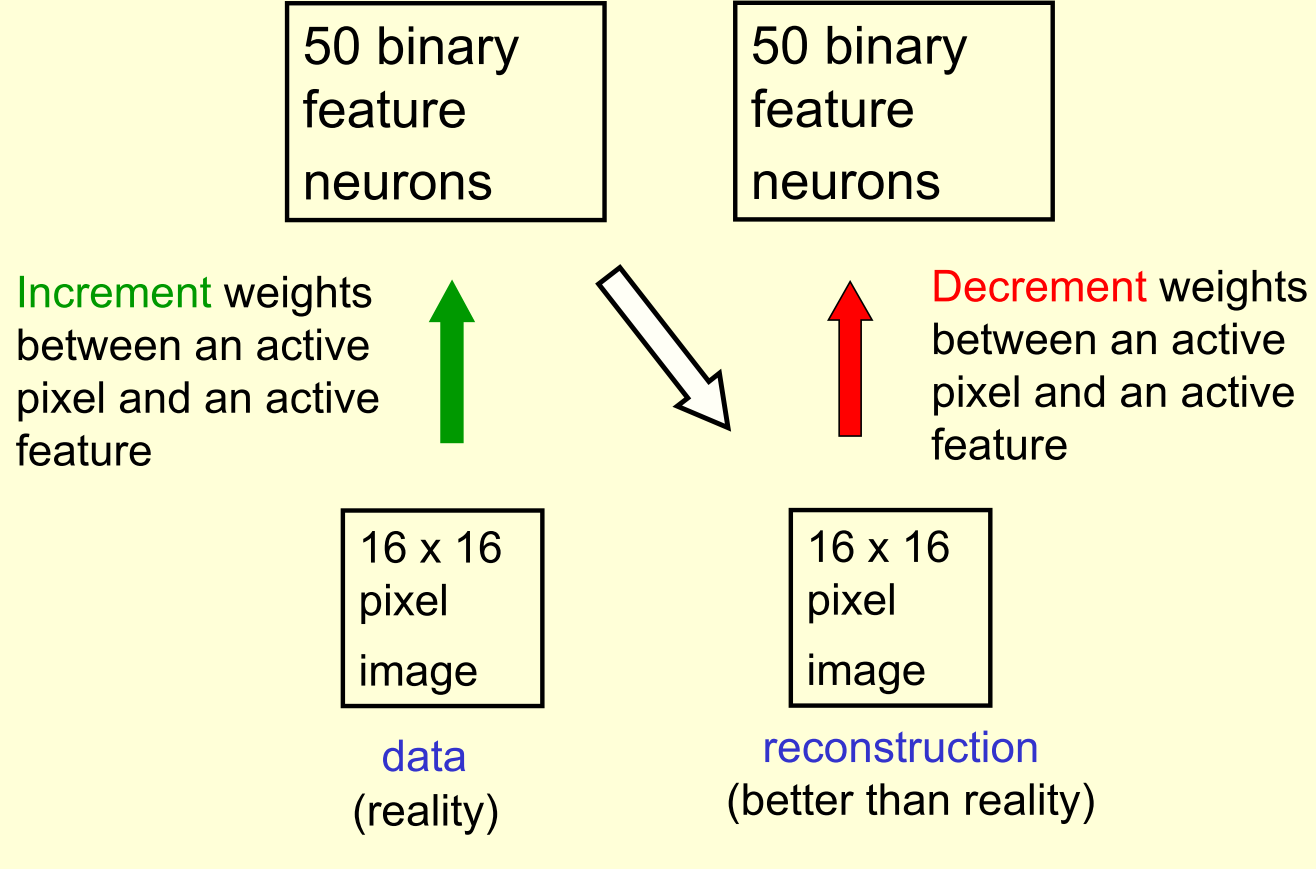
\includegraphics[height=7cm,width=10cm]{reconstruction.png}
        \label{fig:viterbi}
      \end{figure}
}

\frame{
\frametitle{训练}
\begin{enumerate}
\item 先训练一个隐含层,从可见层直接接收数据
\item 在将隐含层的输出作为下一层的可见节点,在进行训练
\end{enumerate}
}

\frame{
\frametitle{产生数据}
   \begin{columns}
    \begin{column}{0.4\textwidth}
      \begin{figure}
        \centering
        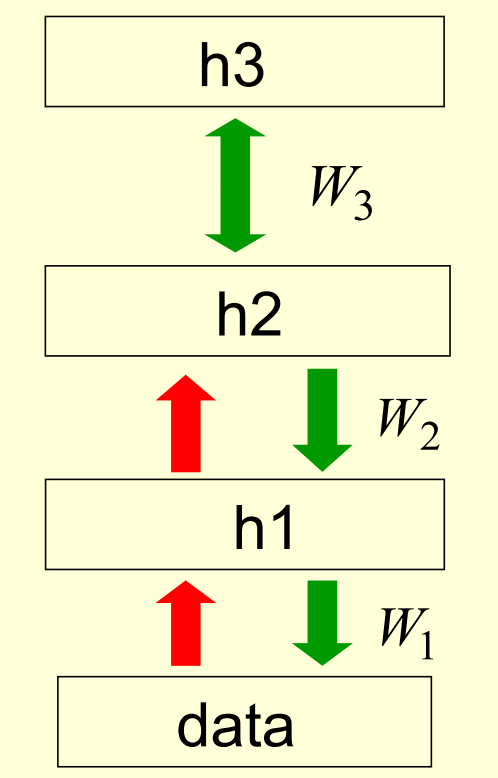
\includegraphics[height=5cm,width=4cm]{gdata.png}
        \label{fig:viterbi}
      \end{figure}
    \end{column}
    \begin{column}{0.6\textwidth}
      得到数据
      \begin{itemize}
      \item 在最上层进行Gibbs sampling,得到$h_2$
      \item 对于其他层,根据分布$P(h^{k-1}|h^k)$进行采样
      \item 最后得到的$x=h^0$即为所得
      \end{itemize}
      最后几个不是产生式模型的一部分,只是用来进行inference的
    \end{column}
  \end{columns}
}

\frame{
  \frametitle{为什么学习方法有效}
  \begin{columns}
    \begin{column}{0.4\textwidth}
      \begin{figure}
        \centering
        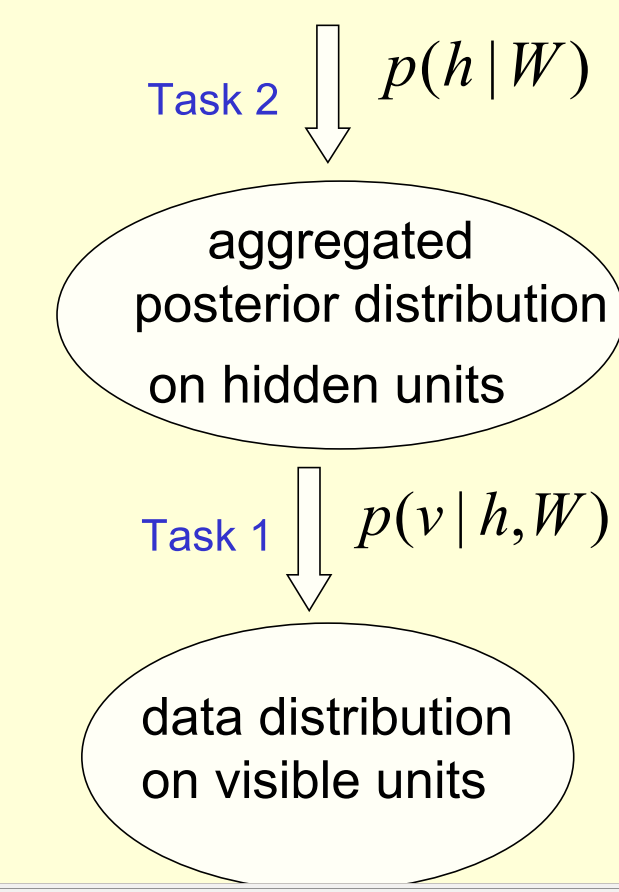
\includegraphics[height=5cm,width=4cm]{learningwork.png}
        \label{fig:viterbi}
      \end{figure}
    \end{column}
    \begin{column}{0.6\textwidth}
      \begin{itemize}
      \item RBM将数据分布转移到隐含层分布
      \item 将任务转化成两步:学习$P(h|W),P(v|h,W)$
      \item 通过第二步modeling数据更容易,因为其更贴近RBM所能model的
      \item RBM能表示为$P(v) = \sum_h p(h)p(v|h)$,对于$P(h)$提高,自然可以提高$P(v)$
      \end{itemize}
    \end{column}
  \end{columns}
  
}

\frame{
\frametitle{例子}
      \begin{figure}
        \centering
        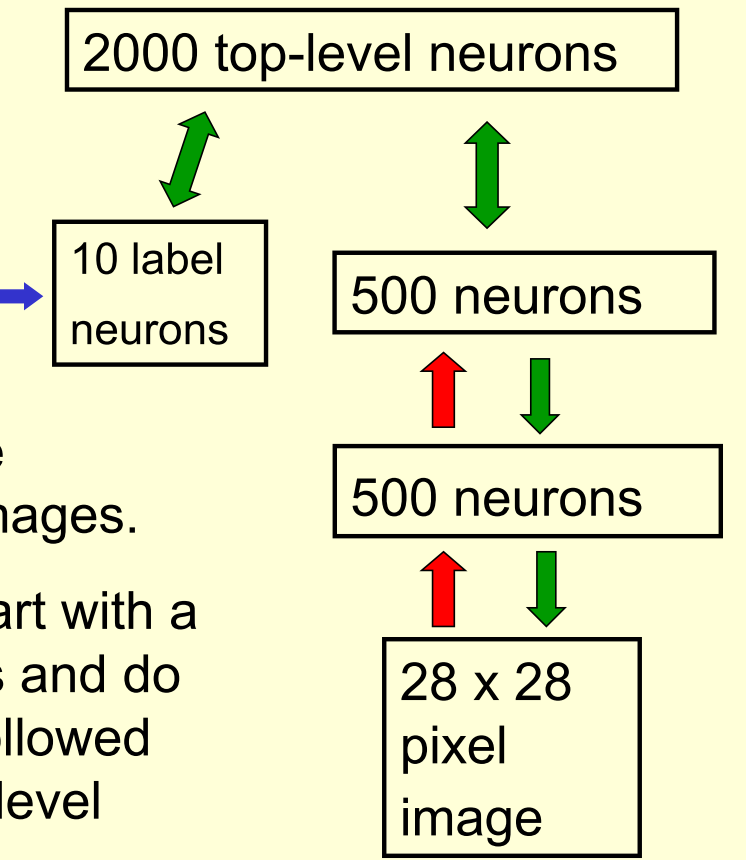
\includegraphics[height=7cm,width=6cm]{digit.png}
        \label{fig:viterbi}
      \end{figure}
}


\end{document}
